% CREATED BY DAVID FRISK, 2016
\chapter{Methods}
\todo{REWRITE TO PAST TENSE}
I am working with AI Habitat, a simulation platform for working with embodied AI\cite{habitat19iccv}. It consists of two parts, Habitat-Sim, the 3D simulator, and Habitat-Lab, the library for embodied AI development. 

\subsection{The Model}
I am starting with the Embodied Question Answering baseline in Habitat-Lab, which consists of three parts, a CNN for initial feature extraction, a question answering module, and a navigation module, called PACMAN\cite{embodiedqa}.
The CNN feature extractor is trained on three tasks: RGB reconstruction, semantic segmentation, and depth estimation.
The question answering module is given the last five frames of navigation (in training taken during ground-truth shortest path navigation), and then predicts an answer from a set of possible answers. 
The navigation is trained via imitation learning to imitate shortest path navigation. \todo{Maybe include an example of the json for an episode?} % SD 2021-05-01 15:07:05 +0200: Imitation learning here is used to distinguish it from reinforcement learning. However, in my underastanding, imitation elarning is just standard ML.
The training of the Habitat-Lab version of the model differs somewhat to the version presented in the Embodied Question Answering paper. For the original model, the CNN, question answering, and navigation modules were all trained separately, and then reinforcement learning was used to fine-tune, and more strongly link the question answering and navigation modules, by using accurate question answering % SD 2021-05-01 15:13:19 +0200: the success of, i.e. yes/no but no more information than this
as part of the reward for the navigation module. This reinforcement learning is missing from the habitat version of the model; the components of the model are only trained separately. 

% SD 2021-05-01 15:14:03 +0200: Reference to the Habitat-Lab github. Reverse the order of descriptions: navigation before QA

% SD 2021-05-01 15:21:10 +0200: Here it would be in place to include a model diagram and then indicate in what ways the baseline model is different from the original Das paper. Later on you can use modified version of the same diagram to point our your extensions. It would also be good to mention the paramateres of the model, i.e. the sizes of inputs, outputs and the intermediate layers.


\section{The Datasets}
\todo{REWRITE TO PAST TENSE} % SD 2021-05-01 15:15:54 +0200: Present tense is okay since this a description of the current research; normally we would use past tense to distinguish what we are doing here from the previous publication.
I am using the Matterport3D dataset, a dataset of real interiors with human annotation of objects, as my scene dataset\cite{matterport}. 
I am using the MP3D-EQA task dataset, which was created using code to automatically generate questions and answers to correspond with annotated scenes in the Matterport3D dataset\cite{eqa_matterport}. 

% SD 2021-05-01 15:14:59 +0200: Reference to git repository.

\subsection{Interiors}

\subsection{MP3D-EQA Dataset} 
This dataset contains questions of three types: 'color\_room': \emph{What color is the <obj> in the <room>?}, 'color': \emph{What color is the <obj>?}, and 'location': \emph{What room is the <obj> located in?}. This dataset was based off of the EQA-V1 dataset\cite{embodiedqa}. There were some differences between the datasets, however. The EQA-V1 dataset included a fourth type of question, prepositional questions: \emph{What is <on/above/below/next to? the <obj> in the <room>?}, but these are not present in MP3D-EQA, due to limited occurence of these relationships in the Matterport3D dataset. % SD 2021-05-01 15:17:33 +0200: I'm not sure if I udnerstand. One can create relations between any two objects.
EQA-V1 was built based on the SUNCG dataset, which is no longer available. % SD 2021-05-01 15:18:04 +0200: Mention earlier that this was used in the original paper.
The paper which introduces the MP3D-EQA dataset was mainly focused on the navigation aspect of the task, and the question types reflect that. A color or location question should theoretically be a good indication of whether or not the agent has successfully navigated to the object, but actually answering the question may not require as complex of reasoning. \todo{discussion of difficulty of color recognition}

\begin{table}[h]
\centering
\caption{Question Type Breakdown}
\begin{tabular}{ |l|l|l| }
\hline
\textbf{question type} & \textbf{percentage of training set} & \textbf{percentage of evaluation set} \\
\hline
color\_room & 69.85908 & 68.46154\\
color & 15.91858 & 17.69231\\
location & 14.22234 & 13.84615\\
\hline
\end{tabular}
\label{tab:q_breakdown}
\end{table}

The dataset has a fixed train/eval split. There is one object which only occurs in the validation set ('toaster'), and one answer that only occurs in the validation set ('gym'). 


% SD 2021-05-01 15:31:45 +0200: The following text should go into a separate section which would be describing our research questions and the experiments to answer them: a good way of doing this is to direct the discussion in the previous secitons in such a way that a reader would have a clear idea what the open questions are (directed by you of course) so that your research questions follow naturally.

\section{Experiment 1: Baseline and Blindfolding}
\label{sec:exp_1}
In this task, I trained and evaluated my baseline model, the CNN and VQA portions of the EQA baseline in habitat-lab. A diagram of the VQA model can be seen in Fig.~\ref{fig:baseline_model}. I also conducted a blindfolding test, in which during evaluation the model was given zeroes instead of the visual information for the scene. This was done by duplicating and modifying the method that converts the .jpgs into numpy arrays to be input to the model, so that it produced an array of zeroes of the same size instead, sending a black/blank image as the input to the model. The point of this blindfolding was to determine if the VQA model was considering the visual input when answering the questions. 

% SD 2021-05-01 15:33:59 +0200: Start with the question first and then describe the exepriment. Discuss also that there are several ways of conducting a blindfold study. For example, the Das et al paper that Nikolai found was changing the architecture of the model and was only using textual information. Why did you choose your method (compared to the other) and what are its implications on results: we test something else, right.

\begin{figure}[h]
     \centering
%     \includegraphics[width=.5\textwidth]{/home/yasmeen/Desktop/thesisproj/thesis/figure/baseline_diagram.png}
     \includegraphics[width=.5\textwidth]{./figure/baseline_diagram.png}
     \caption{VQA Model}
     \label{fig:baseline_model}
\end{figure}

\section{Experiment 2: Basic Semantic Categories}
\label{sec:exp_2}
The agent in habitat-sim includes a 'semantic sensor', that reads annotations from the dataset. It reads annotations of object instances, which can then be mapped to category ids. The list of category IDs can be found in appendix~\ref{app:categories}. These category IDs were used as another information source for the model, as shown in Fig.~\ref{fig:category_model}.

% SD 2021-05-01 15:37:23 +0200: Why do we believe semantic segmentation will be helpful? Also, point out that the categories for semantic segmentations are just general labels for surfaces and objects and than QA on object requires more detailed semantic information about the objects, including common sense knowledge that you mentioned earlier. Why place semantic segmentation after the linguistic and perceptual attention? What are our hypotheses?

\todo{Give more detail on shaping, add motivation}
\begin{figure}[h]
     \centering
%     \includegraphics[width=.75\textwidth]{/home/yasmeen/Desktop/thesisproj/thesis/figure/model_w_semantic.png}
     \includegraphics[width=.75\textwidth]{./figure/model_w_semantic.png}
     \caption{Model With Semantic Category IDs as 3rd input}
     \label{fig:category_model}
\end{figure}

